\subsection{Decision making in a bureaucracy\label{sec:decision-making}}

Decisions are central to the operation of a bureaucratic organization. Although it is worth exploring the topic, it is useful to keep in mind that decisions are not the only source of change in an organization. Occasionally events unfold without decisions being made. This might be because the decision makers are not informed, or there is an \href{https://en.wikipedia.org/wiki/Willful_blindness}{intentional neglect}. This section focuses on situations where bureaucrats recognize the need for a decision and want to make the best decision.

There are multiple types of decisions. 
A \gls{simple decision} has one correct or beneficial choice and one or more wrong or harmful choices. The work of decision making is then to gather information that identifies which is the correct or beneficial choice and select that option.

The best case scenario for any decision making is one person making a well-informed simple decision that has immediate consequence and the consequence is to the decision maker. Examples from elementary formal education include arithmetic math problems, multiple choice quizzes, spelling tests, and memorization tests. A bureaucrat's \href{https://en.wikipedia.org/wiki/Moral_injury}{moral injury} can come from decision making that involves multiple people, weak feedback loops with high latency, and complex decisions for multiple objectives.

\subsubsection{Example Decision Method: Pareto Frontier\label{sec:pareto}}

A complex decision may have many choices, and there are might not be a best option. Then a \href{https://en.wikipedia.org/wiki/Pareto_front}{Pareto frontier} might exist where trade-offs can be made. 

As an example of a complex decision made by one person with immediate consequence and direct relevance to the decision maker, suppose you want to purchase a car. You care about only two aspects: fuel efficiency and cost. See Figure~\ref{fig:pareto_frontier_cars} for an example of the Pareto frontier.

\begin{figure}[ht]
    \centering
    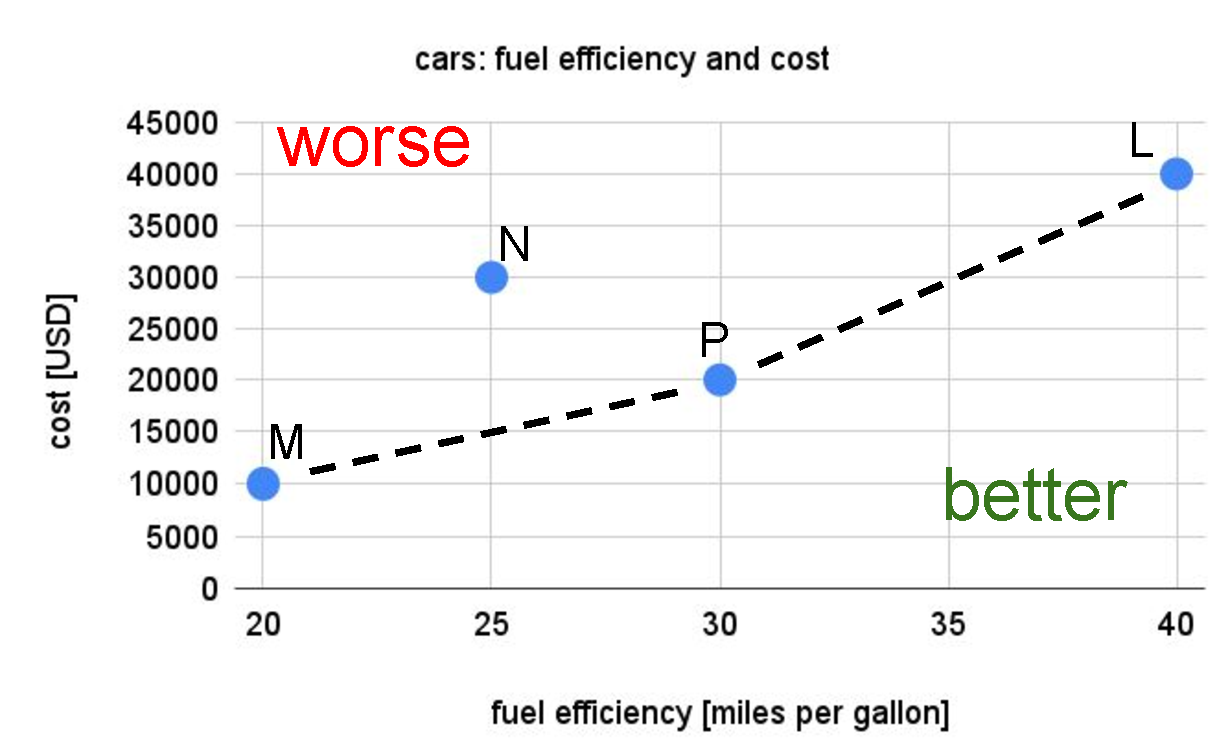
\includegraphics[width=1\textwidth]{images/pareto_frontier_car_options.pdf}
    \caption{Four cars, L, M, N, and P. The goal of the buyer is to spend less money and get better fuel efficiency. Choices not on the frontier should be avoided, but that doesn't yield a single result.}
    \label{fig:pareto_frontier_cars}
\end{figure}

Visualizing a Pareto frontier for two quantitative variables is easy, but typically decisions involve more factors. For example, evaluating the trade-off of three quantitative variables like speed, accuracy, and cost creates a surface. With more than three variables visualization are less useful, though the analysis technique still applies. 

Another constraint on using Pareto frontier analysis is that it works well when there are many options relative to the number of variables being optimized for. 
The assessment does not work as well when there are few choices relative to the number of variables. For example, suppose there are 10 choices of car and you want high fuel efficiency, sufficient cargo capacity, maximum number of passengers, stylish, low cost, low maintenance, good durability, and high resale value. 

For a set of quantitative variables, a Pareto frontier does not account for the relative importance of different variables. Assigning weights to each of these factors merely stretches one axis relative to the other axes. 

There are many possible decision making frameworks besides Pareto frontiers, but in practice a typical bureaucratic decision is ill-informed, has diffuse consequences, delayed impact, and does not affect the decision maker. In bureaucratic processes there is rarely a formal assessment of options. 
Decisions are rarely recorded. 
Even afterwards a decision can be difficult to evaluate for correctness because there are multiple stakeholders.

If the people you want to convince are not swayed by data, then you can augment the cost-benefit analysis with stories. 

\subsubsection{Risks of Using Decision Frameworks}

Decision making frameworks can be attractive to bureaucrats intending to formalize processes (see \S\ref{sec:process}) and encourage predictability. There are potential risks worth being aware of. 

Cost-benefit analysis can decrease the apparent responsibility of the decision maker. Cost-benefit analysis can be used to deflect criticism for an action. 

% https://graphthinking.blogspot.com/2019/01/political-decisions-versus-science.html
A decision is political when the basis is historical relationships, maintenance or creation of a relationship, or to enable future relationships. A decision is subjective when someone else faced with the same scenario would have come to a different conclusion.
A decision is quantitative when it is based on measurements. To avoid the appearance of subjective decision making or political decision making, a decision may be framed as ``data driven." 
% https://graphthinking.blogspot.com/2018/06/data-driven-decisions-versus-data.html
A good approach for data driven quantitative analysis involves coming up with a testable hypothesis, then performing experiments and collecting data to evaluate the hypothesis. More commonly, a decision is made, then data is gathered which supports the desired outcome. Forming an opinion and then looking for evidence to back the outcome yields suboptimal results for the organization.

Even when a bureaucrat is not intentionally biased towards an outcome, there are many ways to gather evidence. Some approaches have biased sampling and produce biased results.

Even with valid and representative data measurement, decision makers can be led astray by poor modeling. A model may use inapplicable techniques, or may have implementation bugs.

For all the dangers of decision making methods, there are worse approaches that do not rely on measurement. People rely on history (if they are aware of it) and perpetuate bad ideas, or take action based on what is best for their career, or decide based on how to accumulate more power, or simply choose based on what someone else says to do.  

\subsubsection{Alternative Decision Making Approaches}
Identifying the spectrum of ways bureaucrats make decisions can decrease the surprise when you encounter these in practice. Enumerating the choices of how to make decision allows for conversation about the pros and cons of each. The spectrum below is ordered from least effective to most effective and is not exhaustive.
\begin{itemize}
    \item Random selection from the options (e.g., roll of the dice, shake the Magic 8 ball -- Fig.~\ref{fig:magic8ball}).
    \item Rely on a hunch.
    \item Rely on past experience, whether your own or someone else's.
    \item Use a cost-benefit model, gather data, analyze.
    \item Make a hypothesis, design an experiment, carry out a test, collect data, analyze.
\end{itemize}

\begin{figure}
    \centering
    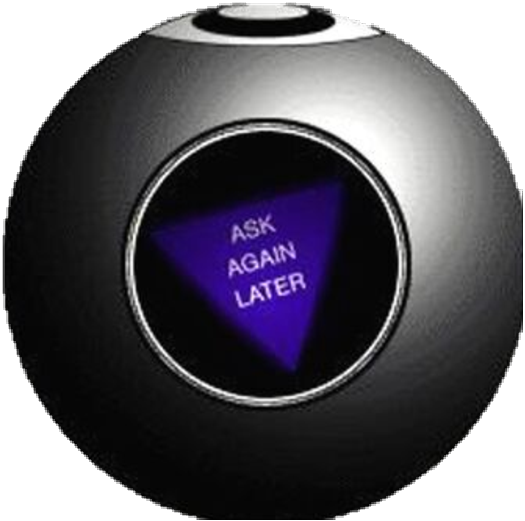
\includegraphics[width=0.4\textwidth]{images/magic8ball.pdf}
    \caption{Magic 8 ball for decision making.}
    \label{fig:magic8ball}
\end{figure}

\subsubsection{Reasons why cost-benefit analysis models are not used}

Applying quantitative models to decision making may seem a useful path to optimal outcomes. Improved decision making that benefits stakeholders seems attractive. There are a variety of reasons this approach is not taken. I will outline the reasoning here not driven by cynicism, but so that you can appropriately respond when confronted with arguments against cost-benefit modeling. Decreasing your surprise through the inoculation of exposure enables you to develop counter-arguments. 

One reason to avoid cost-benefit modeling is that there is a lot of work to do, so coming up with a model is an opportunity cost. Modeling every decision in detail is unrealistic, so triage is needed -- which decisions warrant the investment of analysis. A person inexperienced in modeling of decisions will take longer and is more likely to create a bad model. Practice is expensive. Identifying relevant parameters for inclusion is a learnable skill. 

If a person has a bad experience with cost-benefit modeling, they may be less likely to try again with new decisions. Bad experiences can come from using incorrect data, missing a critical variable, picking the wrong scope for a question, implementing the right model with the wrong math, misinterpreting the result, using a model that is too in-depth or not sufficiently deep, or failing to sell the result of an analysis to stakeholders.

Quantitative cost-benefit modeling doesn't account for personalities or organizational politics. The best options may decrease the decider's power or prestige, or harm relationships. 

To inform a cost-benefit analysis, measurements are needed. In addition to measurement being costly, measurements get perverted -- see \href{https://en.wikipedia.org/wiki/Campbell\%27s_law}{Campbell's law}. \marginpar{[Tag] Folk wisdom}

\subsubsection{Decision Making Delay\label{sec:decision-delay}}

What appears from the outside as ``organizational inertia'' is internal delay of decision making and the delay of dissemination. 
Delay comes from
\begin{itemize}
    \item Time used by each decision maker to gather information, arrive at a decision, modify processes, disseminate their selection, justify their selection. 
    %\item Forcing a continuous variable into a discrete set of choices. Typically the number of choices is small. Discrete choices for a continuous variable is a loss of effectiveness.
    % https://dynomight.net/teaching/
    \item Processes designed to account for cheaters and people with malicious intent, whether that means a malicious bureaucrat or malicious subject. 
\item Analysis paralysis, due to {insufficient information, too much information, which framing is unclear}
\item When other people who are needed to carry out the action push back, either in disagreement or seeking clarification. The fact that the organization is not profit driven is important because the justification for the action isn't quantitatively obvious. Therefore there's a higher burden for communication.
\end{itemize}


% The following characterization has no consequence
% Decision making by bureaucrats can be informal or formal, consensus-based or solo. 


\subsubsection{A Bureaucratic Decision involves many Decisions}

A decision is actually a collection of dependent choices. After recognizing the need for a decision, follow-on decisions include identifying the stakeholders (who to include in an impact analysis) and identifying options. Who is a stakeholder and what are the options are interrelated. Involving more people expands the number of options and the complexity. Additional choices associated with reducing uncertainty are how much time to spend on the decision, how much information to gather for the decision, whether the make the decision or push the decision to someone with more expertise, whether to push the decision to someone with more exposure to the consequences.

Most decisions you make as a bureaucrat do not have hard deadlines. Instead, there are trade-offs in allocation of your time. Sooner is preferable since the consequence of the decision benefits the organization and allows you to focus on other tasks, but delaying allows for more information gathering for a better informed decision. (See Dilemma~\ref{table:gather_data_lots-vs-little} and other related Dilemmas in that section.)


If a bureaucrat is going to rely on expert consultation (see \S\ref{sec:expertise} on expertise), the decision maker needs to be confident the expert is not of straying outside their area of expertise. For example, I don't rely on a botanist with many published papers to tell me how to change the oil in my car. 
Besides knowing their own limitations, the expert should be clear about whether their input is a factual summary, a predictive assessment, or a value judgement. This nuance complicates what you as a bureaucrat are interested in (what's the best choice?).


\subsubsection{Transparency of Decision Making\label{sec:transparency-of-decisions}}

Your decision making process might change if made visible to stakeholders. You may provide clearer justifications, or spend more time gathering evidence to support a claim. Strengthening the arguments is beneficial but takes time and resources. 

Frank conversations and exploratory brainstorming need protections to allow participants to be vulnerable. This is the motive for the \href{https://en.wikipedia.org/wiki/Chatham_House_Rule}{Chatham House Rule}. At the same time, people impacted by the decisions benefit from understanding how the decisions were made -- see examples like 
\href{https://en.wikipedia.org/wiki/Government_in_the_Sunshine_Act}{Sunshine laws} and \href{https://en.wikipedia.org/wiki/Freedom_of_Information_Act_(United_States)}{FoIA}. Even the symbolism of survelince changes behavior
\footnote{K.~J.~Haley and D.~Fessler (2005). ``Nobody’s watching? Subtle cues affect generosity in an anonymous dictator game.'' Evolution and Human Behavior, 26, 245–256.\\
T.~Burnham and B.~Hare (2007). ``Engineering human cooperation.'' Human Nature, 18, 88–108.}.

Making decisions transparently can make participants more risk averse because of the potential for failure. 

The concept of transparency can apply before a decision is issued, while a policy is in effect, or after the consequence (as part of a review). 